\documentclass[11pt]{article}
\usepackage[T1]{fontenc}
\usepackage{lmodern}
\usepackage[a4paper,margin=27mm]{geometry}
\usepackage{amsmath,amssymb,amsthm,booktabs,graphicx,tikz}
\usepackage{microtype}
\usepackage[numbers,sort&compress]{natbib}
\usepackage[hidelinks]{hyperref}
\setlength{\emergencystretch}{2em}
\newtheorem{theorem}{Theorem}
\newtheorem{lemma}[theorem]{Lemma}
\newcommand{\ket}[1]{|#1\rangle}
\newcommand{\bra}[1]{\langle#1|}
\newcommand{\Id}{\mathbb I}
\newcommand{\norm}[1]{\lVert#1\rVert}
\newcommand{\HH}{\mathcal H}
\title{Near-star spectral gaps on subdivided two-star qubit networks}
\author{Xiaojian Zeng\\[2pt]
\small PBC School of Finance, Tsinghua University, 100190\\
\small \href{mailto:xiaojianzeng@foxmail.com}{xiaojianzeng@foxmail.com}}
\date{}
\begin{document}
\maketitle
\begin{abstract}
We determine the lowest excitation of an unweighted qubit network whose
edges favor the unnormalized pair state $\ket{00}+s\ket{11}$. The graph
consists of two hubs, each with $k$ private leaves, joined through one
shared vertex. For every integer $k\geq100$ and every
$\theta\in[1/2,2]$, with $1-s^2=\theta/k$, the full ground and first
excited energies are simple. Their gap satisfies
$\Delta/(1-s^2)=1+1/(2k)+(1-\theta)/(4k^2)+R$, with
$|R|\leq364/k^3$. In particular, the gap exceeds $1-s^2$ throughout
this domain and approaches that star-graph threshold uniformly on an
infinite nonstar family. A full-star operator inequality controls all
higher number sectors, while a separate Weyl bound excludes every
internal competitor in the ground sector. Exact rational polynomial
bounds and root isolation identify the two relevant eigenvalues and
control the expansion. The limit has growing hub degree and fixed edge
strength; it does not establish a bounded-degree thermodynamic result
or resolve the sharp-gap conjecture for arbitrary graphs and parameters.
\end{abstract}

\section{Model and relation to existing gap bounds}

For a finite connected simple graph $G=(V,E)$ with one qubit per vertex,
consider the time-independent closed-system Hamiltonian
\begin{equation}
 H_s(G)=-\sum_{\{i,j\}\in E}
 (\ket{00}+s\ket{11})(\bra{00}+s\bra{11})_{ij},
 \qquad 0\leq s<1 .
 \label{eq:model}
\end{equation}
Every term has identity spectators. The common edge energy is $J=1$;
for $J>0$, all energies and gaps below scale by $J$. The parameter $s$
is dimensionless. No edge phases, additional fields, weights, auxiliary
systems, bath or drive are introduced. Connections and boundary
conditions are specified entirely by $G$. The local ket is
\emph{unnormalized}: normalization would divide the spectrum and the
gap by $1+s^2$.

Wong, Bravyi, Gosset and Liu introduced this deformation and proved the
star gap $1-s^2$ for at least three vertices
\cite[Section 5.5, Lemma 13]{Wong2026}. They conjectured
$\Delta(H_s(G))\geq1-s^2$ for all connected graphs and all $s<1$
\cite[Conjecture 3]{Wong2026}. Here the full spectrum, with
multiplicity, is ordered as $E_0\leq E_1\leq\cdots$, and
$\Delta=E_1-E_0$. The separate conjecture that the first excitation is
odd is not assumed.

In the convention $Z\ket{0}=\ket{0}$, $Z\ket{1}=-\ket{1}$, the positive
local term is
\begin{equation}
 \frac{1+s^2}{4}(\Id+Z_iZ_j)
 +\frac{1-s^2}{4}(Z_i+Z_j)
 +\frac{s}{2}(X_iX_j-Y_iY_j).
 \label{eq:pauli}
\end{equation}
Thus the minimum-field theorem for Suzuki--Fisher Hamiltonians
\cite[Theorem 1]{Bravyi2026} implies
\begin{equation}
 \Delta(H_s(G))\geq \frac{d_{\min}(G)}{2}(1-s^2),
 \label{eq:prior}
\end{equation}
because the intrinsic field at vertex $i$ is $d_i(1-s^2)/4$.
The sharp conjectured threshold already follows when $d_{\min}\geq2$;
the degree-one case retains a factor of two in this bound
\cite[Section 5.4]{Wei2026}. Other Lee--Yang results provide an
added-field gap bound \cite[Theorem 11]{Rayudu2026} and, for
\eqref{eq:model}, the bound $(1-s^2)/2$
\cite[Theorem 6.10]{Hofgard2026}. Positive-gap algorithmic results are
therefore established prior work, rather than a consequence first
obtained here. At the excluded endpoint $s=1$, $H_1=-2Q$, where $Q$
is the positive sum of normalized EPR projectors studied by Ju and
Nagda \cite{Ju2025}.

The present calculation determines the actual full gap, including its
first relative corrections, on a particular infinite family with leaves.
It uses standard symmetry and Perron reductions. Wong's thesis already
develops orbit reduction for stoquastic Hamiltonians, including ordinary
double stars whose hubs are joined directly
\cite[Section 3.3, Theorem 13 and Example 2]{WongThesis2026}.
Our contribution is the full first-excitation ordering and uniform
joint-limit expansion on the subdivided family below. It is not a new
symmetry-reduction method. The comparisons concern the cited statements;
no exhaustive priority claim or resolution of the universal conjecture
is made.

\section{The family and its full spectral gap}

Let $T_k$ have hubs $a,b$, a shared neighbor $c$, private leaves
$u_1,\ldots,u_k$ at $a$, and $v_1,\ldots,v_k$ at $b$. Its only edges are
\begin{equation}
 ac,\ bc,\ au_i,\ bv_i\quad(1\leq i\leq k).
 \label{eq:graph}
\end{equation}
Then $n=2k+3$, $m=2k+2$, and the hubs have degree $k+1$.
Unlike an ordinary double star, their distance is two.

\begin{figure}[htbp]
 \centering
 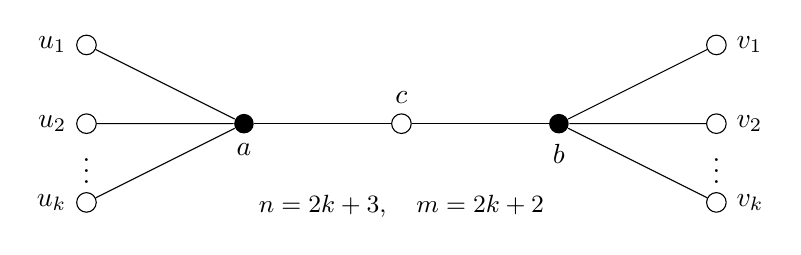
\begin{tikzpicture}[x=1cm,y=1cm,
 hub/.style={circle,fill=black,inner sep=2.5pt},
 site/.style={circle,draw,fill=white,inner sep=2.5pt}]
 \node[hub,label=below:$a$] (a) at (-2,0) {};
 \node[hub,label=below:$b$] (b) at (2,0) {};
 \node[site,label=above:$c$] (c) at (0,0) {};
 \node[site,label=left:$u_1$] (u1) at (-4,1) {};
 \node[site,label=left:$u_2$] (u2) at (-4,0) {};
 \node[site,label=left:$u_k$] (uk) at (-4,-1) {};
 \node[site,label=right:$v_1$] (v1) at (4,1) {};
 \node[site,label=right:$v_2$] (v2) at (4,0) {};
 \node[site,label=right:$v_k$] (vk) at (4,-1) {};
 \draw (a)--(c)--(b);
 \draw (u1)--(a) (u2)--(a) (uk)--(a);
 \draw (v1)--(b) (v2)--(b) (vk)--(b);
 \node at (-4,-.5) {$\vdots$};
 \node at (4,-.5) {$\vdots$};
 \node[font=\small] at (0,-1.05) {$n=2k+3,\quad m=2k+2$};
\end{tikzpicture}

 \caption{The tree $T_k$. Each hub has $k$ private leaves, and the
 degree-two vertex $c$ is their only shared neighbor. All displayed
 edges carry the same interaction in \eqref{eq:model}; the ellipses
 denote the remaining private leaves.}
 \label{fig:tree}
\end{figure}

Put $q=s^2$, $\eta=1-q$, and $U=X_aX_b$. The operator
\begin{equation}
 B=-UH_s(T_k)U
 \label{eq:B}
\end{equation}
is positive semidefinite and preserves ordinary occupation number $N$
in this transformed basis. Denote the largest eigenvalue of its
\emph{complete} number sector by $\lambda_N$. This definition does not
restrict to permutation-symmetric states.

\begin{theorem}
For every integer $k\geq100$ and every real $\theta\in[1/2,2]$, set
$\eta=\theta/k$ and $s=\sqrt{1-\eta}$. The full ground and first
excited energies of \eqref{eq:model} on $T_k$ are simple and equal to
$-\lambda_2$ and $-\lambda_3$, respectively. They satisfy
\begin{equation}
 \left|\frac{\Delta(H_s(T_k))}{\eta}
       -\left(1+\frac1{2k}+\frac{1-\theta}{4k^2}\right)\right|
 \leq\frac{364}{k^3}.
 \label{eq:gap}
\end{equation}
In this whole domain $\Delta>\eta$, and $\Delta/\eta$ tends uniformly
to one as $k\to\infty$. Every full sector $N\geq4$ obeys
\begin{equation}
 \lambda_N<\lambda_3-\frac{(N-3)\eta}{2}.
 \label{eq:tail}
\end{equation}
The original-gauge ground state is even and the first excitation is odd.
\label{thm:gap}
\end{theorem}

The proof has two distinct ingredients. Exact low-sector calculations
identify $\lambda_2,\lambda_3$ with uniform errors. Full-space operator
bounds then show that no other sector or internal ground-sector mode
can compete with them. A difference of two chosen-sector trial energies
would not suffice for the theorem.

\subsection{Number convention and sector maxima}

Each edge is oriented with its hub first. The hub flip maps its positive
ket to $\ket{10}+s\ket{01}$, so the nonzero local matrix of $B$ is
\begin{equation}
 \begin{pmatrix}1&\sqrt q\\ \sqrt q&q\end{pmatrix}_{10,01}.
 \label{eq:local}
\end{equation}
This is a unitary change of physical basis. Number conservation in this
basis does not imply ordinary number conservation for $H_s$ in the
original basis. Two hub flips preserve the original parity
$\bigotimes_i Z_i$.

For $q>0$ and $0<N<n$, the full $N$-occupation matrix is nonnegative
and irreducible. Exchanges along the edges of a connected graph connect
all $N$-subsets: holes can be moved along paths on a spanning tree to
relocate tokens successively. Perron--Frobenius therefore gives a simple
largest eigenvalue and a strictly positive vector in each such sector.
Uniqueness makes that vector invariant under the two private-leaf
permutation groups and under branch reflection. Hence the sector
\emph{maximum} can be computed in the leaf-symmetric, reflection-even
block. No statement about an internal second eigenvector follows from
this observation; those modes are bounded separately below.

\section{Low-sector roots with uniform error control}

\subsection{Exact rational quotients}

An occupation orbit is labeled by $(\alpha,\beta,\zeta,p,r)$, where
$\alpha,\beta,\zeta\in\{0,1\}$ are the hub and middle occupations,
$p,r$ are the private-leaf counts, and
$\alpha+\beta+\zeta+p+r=N$. Write amplitudes on each orbit as
$s^{\alpha+\beta}$ times a constant. This positive similarity gives
a rational quotient $Q_N$ in $k,q$. Its diagonal is
\begin{align}
 (Q_N)_{vv}&=f(\alpha,\zeta,p)+f(\beta,\zeta,r),\label{eq:diag}\\
 f(\alpha,\zeta,p)&=\alpha(1-\zeta+k-p)
                    +(1-\alpha)q(\zeta+p).\nonumber
\end{align}
Its private-leaf row transitions are
\begin{equation}
 (1,p)\longrightarrow(0,p+1):\ k-p,\qquad
 (0,p)\longrightarrow(1,p-1):\ qp,
 \label{eq:private}
\end{equation}
with the other branch unchanged. For a hub--middle exchange the row
coefficients are $1$ from $(1,0)$ and $q$ from $(0,1)$. Terms whose
target occupancy is not allowed are absent. The positive diagonal metric is
\begin{equation}
 w_v=\binom{k}{p}\binom{k}{r}q^{\alpha+\beta},\qquad
 WQ_N=Q_N^{\mathsf T}W.
 \label{eq:metric}
\end{equation}
Reflection sends
$(\alpha,\beta,\zeta,p,r)$ to $(\beta,\alpha,\zeta,r,p)$.
For its even block, each row is summed over target reflection orbits;
the orbit's cardinality multiplies its metric weight. The unfurled
dimensions are $12$ and $20$ for $N=2,3$, and reflection reduces them
to $7$ and $11$. Equations \eqref{eq:diag}--\eqref{eq:metric} specify
every matrix entry without a fitted or numerical input. The positive
metric also applies to auxiliary real $k\geq100$, since the binomial
products used here have $p,r\leq3$.

\subsection{Rational polynomial enclosures}

Let $\chi_N(x;k,q)=\det(x\Id-Q_N)$ for the reflection-even quotient.
Set $e=1/k$, $q=1-\theta e$, and substitute
\begin{equation}
 x=\frac2e+4+e(h-N\theta).
 \label{eq:scaled}
\end{equation}
Remove the lowest Laurent power of $e$ from the substituted determinant,
calling the resulting polynomial $P_N(e,\theta,h)$. Direct exact
calculation gives
\begin{equation}
 P_2(0,\theta,h)=8h,\qquad P_3(0,\theta,h)=32h.
 \label{eq:leading}
\end{equation}
The polynomials, matrices and their exact rational coefficient bounds
are supplied with the reproduction code.

The bounds use the box
$0\leq e\leq1/100$, $1/2\leq\theta\leq2$, $|h|\leq1$.
For a polynomial $F=\sum c_{ijl}e^i\theta^j h^l$, its coefficient norm
\begin{equation}
 \mathcal C(F)=\sum_{i,j,l}|c_{ijl}|100^{-i}2^j
 \label{eq:norm}
\end{equation}
is a uniform upper bound for $|F|$ on this box. All coefficients
and all operations in this norm are rational. Define the truncations
\begin{align}
 \bar h_2&=-2e+(2\theta+10)e^2,\label{eq:h2}\\
 \bar h_3&=-\frac{\theta+4}{2}e
              +\frac{\theta^2+7\theta+40}{4}e^2.\label{eq:h3}
\end{align}
The exact determinant expansion cancels the residual terms of degrees
zero, one and two. Applying \eqref{eq:norm} to the derivative deviation
and to $P_N(e,\theta,\bar h_N)/e^3$ yields the outward rational bounds
in Table~\ref{tab:bounds}.

\begin{table}[htbp]
\centering
\begin{tabular}{@{}ccccc@{}}
\toprule
$N$ & $\deg_x\chi_N$ & $|\partial_h P_N-\ell_N|$
    & $|P_N(e,\theta,\bar h_N)|/e^3$ & $C_N$\\
\midrule
2 & 7  & $<187/200$  & $<572$  & 81\\
3 & 11 & $<1541/250$ & $<2597$ & 101\\
\bottomrule
\end{tabular}
\caption{Uniform exact coefficient bounds, with $\ell_2=8$ and
$\ell_3=32$. The last column bounds the root error by
$|h-\bar h_N|\leq C_Ne^3$, equivalently an eigenvalue error
$C_Ne^4$. The tabulated inequalities round rational bounds outward;
they are not estimates from floating-point sampling.}
\label{tab:bounds}
\end{table}

The derivative lower bounds are $1413/200$ and $6459/250$, respectively.
The residual divided by the derivative lower bound is smaller than
$81e^3$ and $101e^3$. Moreover
$|\bar h_2|\leq107/5000$ and $|\bar h_3|\leq629/20000$ by the same norm.
Adding $C_N/100^3$ keeps both error neighborhoods inside $|h|<1$.
Strict monotonicity and the intermediate-value theorem thus give a
unique simple real root in each enclosure.

It remains to identify these roots as the sector maxima. At
$(k,\theta)=(100,1/2)$, exact rational root isolation counts all seven
and eleven roots, including multiplicities, and identifies the enclosed
roots as the largest simple roots. The second corner $(100,2)$ supplies
an additional exact check. Their gap enclosures are reported in
Table~\ref{tab:anchors}. These are complete quotient-root counts, rather
than an iterative eigensolver's selected roots.

For auxiliary real $k\geq100$, the positive metric
\eqref{eq:metric} makes all eigenvalues real and continuous. The
parameter domain is connected, and the enclosed root remains simple
everywhere by the derivative bound. It cannot exchange order with
another root without becoming multiple. The one exact anchor therefore
identifies the largest roots on the whole domain. This real-$k$
continuation is algebraic; physical graphs still have integer $k$.
Combining the enclosures with \eqref{eq:scaled} gives
\begin{align}
 \left|\lambda_2-\left(2k+4-\frac{2\theta}{k}
           -\frac2{k^2}+\frac{2\theta+10}{k^3}\right)\right|
 &\leq\frac{81}{k^4},\label{eq:lam2}\\
 \left|\lambda_3-\left(2k+4-\frac{3\theta}{k}
           -\frac{\theta+4}{2k^2}
           +\frac{\theta^2+7\theta+40}{4k^3}\right)\right|
 &\leq\frac{101}{k^4}.\label{eq:lam3}
\end{align}

\begin{table}[htbp]
 \centering
 \begin{tabular}{@{}cccc@{}}
\toprule
$\theta$ & $\eta$ & Complete root counts $(N=2,3)$ & $\Delta/\eta$ enclosure\\
\midrule
$1/2$ & $1/200$ & $(7,11)$ & $[1.005013181996, 1.005013181997]$\\
$2$ & $1/50$ & $(7,11)$ & $[1.004974283580, 1.004974283581]$\\
\bottomrule
\end{tabular}

 \caption{Exact anchors at $k=100$. Each characteristic polynomial
 has all roots isolated using rational intervals of width at most
 $10^{-24}$, and its enclosed largest root is simple. The displayed
 gap-ratio intervals are rounded outward to twelve decimal places
 from the rational enclosures. Full-space ordering uses the analytic
 bounds in Section~\ref{sec:ordering}, rather than these finite checks.}
 \label{tab:anchors}
\end{table}

\section{Complete-sector ordering}
\label{sec:ordering}

\subsection{A full-star operator inequality}

Let $M_L$ be the positive operator on a star with $L$ leaves, using
the oriented interaction \eqref{eq:local}, and let $N_\star$ be its
occupation number. On the entire star Hilbert space,
\begin{equation}
 M_L\leq(L+1)\Id-\eta N_\star,
 \qquad \eta=1-q,\quad0\leq q\leq1.
 \label{eq:envelope}
\end{equation}
This is a consequence of the star spectrum, whose symmetric form
is established in the source \cite{Wong2026}. To apply it as an
operator inequality we include every nonsymmetric copy and endpoint.

Decompose the $L$ leaf qubits into spin $j=L/2-d$,
$0\leq d\leq\lfloor L/2\rfloor$, with multiplicity
$\binom Ld-\binom L{d-1}$, where $\binom L{-1}=0$.
Each copy has leaf occupations $p=d,\ldots,L-d$. In a paired total-$N$
block, the hub/leaf states $(1,N-1)$ and $(0,N)$ give
\begin{equation}
 M_{d,N}=\begin{pmatrix}
 L-N+1 & \sqrt{q(N-d)(L-d-N+1)}\\
 \sqrt{q(N-d)(L-d-N+1)} & qN
 \end{pmatrix}.
 \label{eq:spinblock}
\end{equation}
This positive matrix has trace $L+1-\eta N$ and determinant
$qd(L+1-d)\geq0$. Each eigenvalue is consequently bounded above by
the trace. The low singleton has hub occupation zero, $N=d$ and
diagonal $qN$; its slack below the same bound is $L+1-N\geq0$.
The high singleton has hub occupation one, $N=L-d+1$ and diagonal
$L-N+1$; its slack is $qN\geq0$. These include the vacuum and
fully occupied endpoints. The spin decomposition exhausts the full
space with its multiplicities, proving \eqref{eq:envelope}.
No irreducibility at $q=0$ or $q=1$ is needed.

\subsection{Every higher number sector}

The two $(k+1)$-leaf stars in $T_k$ overlap only at $c$.
Their number operators add to $N+n_c$. Adding the two valid operator
inequalities \eqref{eq:envelope} gives
\begin{equation}
 B\leq(2k+4)\Id-\eta(N+n_c)
   \leq(2k+4)\Id-\eta N.
 \label{eq:globalenvelope}
\end{equation}
This step does not require the overlapping stars to commute. It
holds for every leaf-spin representation, reflection space and
high-filling endpoint. Thus $\lambda_N\leq2k+4-\eta N$ for every
complete sector.

Dropping the positive $k^{-3}$ term from \eqref{eq:lam3} gives
\begin{equation}
 \lambda_3\geq2k+4-\frac{3\theta}{k}
                    -\frac3{k^2}-\frac{101}{k^4}.
 \label{eq:lam3lower}
\end{equation}
For $N\geq4$, the difference between
$\lambda_3-(N-3)\eta/2$ and the sector envelope is at least
\begin{equation}
 \frac{(N-3)\theta}{2k}-\frac3{k^2}-\frac{101}{k^4}
 \geq\frac1k\left(\frac14-\frac3{100}-\frac{101}{100^3}\right)
 =\frac{219899}{1000000k}>0.
 \label{eq:tailmargin}
\end{equation}
This proves the stronger tail statement \eqref{eq:tail} on the full
Hilbert space, rather than on its permutation-symmetric subspace.

\subsection{Low sectors and internal ground-sector competitors}

Write $B=A+C$, where $A$ is the sum of the two disjoint private
$k$-leaf stars and leaves $c$ free, while $C$ contains just $ac,bc$.
The actual orientation of $C$ has the hubs at $a,b$ and the common
site at $c$. Its full spectra in number sectors one and two are
\begin{equation}
 \operatorname{spec}(C|_{N=1})=\{0,1,1+2q\},\qquad
 \operatorname{spec}(C|_{N=2})=\{0,q,2+q\}.
 \label{eq:C}
\end{equation}
Its zero- and three-occupation blocks are zero, so $\norm C=2+q$
for $0\leq q\leq1$.

The complete one-occupation spectrum of a private star is $k+q$
(simple), $q$ (multiplicity $k-1$) and zero. Its two-occupation
maximum is $k-1+2q$, simple for $q>0$. In total $N=2$ with $c=0$,
$A$ has a unique maximum $2(k+q)$ from private fillings $(1,1)$.
Every other eigenvalue is at most $k+2q$: this includes a
nonsymmetric $q$ leaf mode paired with $k+q$, and the $(2,0)$ or
$(0,2)$ maxima $k-1+2q$. For $c=1$ the private filling is one,
whose maximum is $k+q$. Thus the second largest eigenvalue of the
\emph{full} $N=2$ block of $A$ is at most $k+2q$. Weyl's inequality
then bounds every internal competitor of $B$ in this sector by
\begin{equation}
 \lambda_{\mathrm{second}}(B|_{N=2})
 \leq k+2q+\norm C=k+2+3q\leq k+5.
 \label{eq:internal}
\end{equation}
Likewise $\lambda_1\leq k+2+2q\leq k+4$, while $\lambda_0=0$.
Equation \eqref{eq:lam3lower} gives the uniform separation
\begin{equation}
 \lambda_3-(k+5)
 \geq k-1-\frac6k-\frac3{k^2}-\frac{101}{k^4}
 \geq\frac{9893969899}{100000000}>0.
 \label{eq:lowmargin}
\end{equation}
All multiplicities and nonsymmetric private-leaf modes have therefore
been retained and excluded from competition with $\lambda_3$.

\subsection{Gap and simplicity}

Subtract \eqref{eq:lam3} from \eqref{eq:lam2} and divide by
$\eta=\theta/k$. The total error is at most
$(81+101)/(\theta k^3)\leq364/k^3$, giving \eqref{eq:gap}.
Its excess above one is bounded below by
\begin{equation}
 \frac{\lambda_2-\lambda_3}{\eta}-1
 \geq\frac1{2k}-\frac1{4k^2}-\frac{364}{k^3}
 \geq\frac{4611}{10000k}>0.
 \label{eq:strict}
\end{equation}
In particular $\lambda_2>\lambda_3$. The sector Perron argument,
\eqref{eq:tailmargin}, \eqref{eq:internal} and \eqref{eq:lowmargin}
show that these are exactly the largest two eigenvalues of $B$ in
the complete physical space. Both are simple. Other levels inside
$N=3$ are strictly below its simple Perron maximum; those inside
$N=2$ obey \eqref{eq:internal}. The sign change in \eqref{eq:B}
therefore gives $E_0=-\lambda_2$ and $E_1=-\lambda_3$ with
multiplicity counted. Parity preservation by $U$ makes the original
ground even and the first excitation odd. The uniform error bound
also proves the stated uniform limit. This completes
Theorem~\ref{thm:gap}.

\section{Reproduction and physical interpretation}

The exact supplementary calculation constructs the quotients from
the source Pauli identity and collective-spin ladder factors,
computes the two characteristic polynomials, evaluates rational
coefficient norms, and isolates all anchor roots. Direct physical
number-space matrices at $k=3$, $s=3/5$ intertwine exactly with the
quotients on dimensions $36$ and $84$. These small systems check the
transcription, rather than the universal parameter quantifiers.
As a normalization and sign control, a direct local-ket construction
agrees exactly with \eqref{eq:pauli}; the complete four-qubit star at
$s=1/2$ has $E_0=-13/4$, $E_1=-5/2$ and $\Delta=3/4$, reproducing
the known star law \cite{Wong2026}.

The calculation uses SymPy 1.14.0 for exact polynomial arithmetic
and rational real-root isolation. No approximate eigensolver, fit
or finite graph scan establishes the universal inequalities.
AI assistance was used to develop and check the derivation, generate
and review code, compare primary literature, and prepare the text.
The mathematical basis of the result is the explicit full-space
argument and reproducible exact algebra; the supplementary data
contain the complete matrices, polynomials and rational enclosures.

The lowest excitation of this two-hub network is a number-three
state above the number-two ground state in the hub-flipped basis.
This is a physical parity statement in the original model, not
ordinary original-gauge particle addition. Its energy scale is
$\Delta\sim\theta/k$, with a positive relative excess $1/(2k)$
over the star threshold and a controlled $\theta$-dependent next
correction. Nonstar trees consequently approach the star ratio
within this joint size/endpoint regime. The full-star envelope and
the internal-sector estimate are what make this a prediction for
the actual lowest excitation, including omitted symmetry modes.

The hub degree grows while each edge retains strength $J=1$.
The closing gap along $1-s^2=\theta/k$ is therefore not a
bounded-degree thermodynamic limit, a phase transition, or an
experimental realization claim. We establish neither an all-$s$
result on $T_k$ nor a theorem for general nonstar graphs, arbitrary
weights or phases. General odd-first ordering is not settled.
The original all-graph sharp-gap conjecture remains unresolved by
this family calculation. Existing positive-gap and algorithmic
results retain their separate scope.

\section*{Data and code availability}
The local reproduction package contains the exact certificate
program and its rational outputs, the complete manuscript sources,
and regeneration instructions with the tested environment.
The anchor table is generated from the saved rational enclosures.
Primary papers are identified through bibliographic links; their
full texts are not redistributed with the supplement.

\section*{Acknowledgements}
\paragraph{AI disclosure.}
OpenAI Codex was used for research ideation, derivation assistance,
code generation, exact computational checks, literature retrieval
and manuscript drafting. Its role extended beyond language editing.
This local draft awaits the named author's critical scientific
review, validation of the AI-assisted outputs, and confirmation of
authorship and affiliation. Completed human validation is not asserted.

\bibliographystyle{unsrtnat}
\bibliography{references}
\end{document}
